%%% Choose between 16:9 and 4:3 format by commenting out/uncommenting one of the following lines:
\documentclass[aspectratio=169]{beamer} % 16:9
% \documentclass{beamer} % 4:3

%=========================================================================================================================

\usepackage[ngerman]{babel} % Für neue deutsche Rechtschreibung
\usepackage[utf8]{inputenc}
\usepackage{tikz}               % For creating graphics
\usepackage{url}                % For including urls
\usepackage{tabularx}           % For better tables
\usepackage{colortbl}  % Für \rowcolors und farbige Tabellen
\usepackage{array}     % Für zusätzliche Tabellen-Layouts
\usepackage{xcolor}    % Für Farben

\usetheme{aig}                  % Set beamer theme

%=========================================================================================================================
\title{Stimmungsanalyse mit Twitter}

\author[Team Twitter Sentiment]{Anne Huber, Andreas Franke, Felix Lindner, Burak Özkan, Milomir Soknic}
\institute{Projektpraktikum Web Science,\\Artificial Intelligence Group,\\
University of Hagen, Germany}
\date{18. März 2025}
%=========================================================================================================================
\logo{
\includegraphics[width=3cm]{figures/logoaig.png}}
%=========================================================================================================================

\begin{document}

%=========================================================================================================================

\begin{frame}
  \titlepage
\end{frame}
\nologo

\begin{frame}{Motivation}
  \Large
  \begin{itemize}
      \item Stimmungsanalyse auf Twitter
      \item Besonderheiten von Tweets:
      \item Relevanz für Web Science:
  \end{itemize}
  \vspace{0.5cm}
  \textbf{Zielsetzung}
  \begin{itemize}
      \item Vergleich klassischer ML-Methoden mit Deep Learning für präzisere Stimmungsanalysen.
  \end{itemize}
\end{frame}


%=========================================================================================================================
\section{Daten}


\begin{frame}{Datenauswahl}
  \Large
  \begin{itemize}
      \item Prüfung diverser Datensätze
      \item Entscheidung für \glqq Sentiment140\grqq
      \item Besonderheiten:
      \begin{itemize}
          \item Emojis als Sentiment-Indikatoren
          \item Ausbalancierte Klassen
          \item Bessere Datenqualität
          \item Artikel: \glqq Twitter Sentiment Classification using Distant Supervision\grqq
      \end{itemize}
  \end{itemize}
\end{frame}

\begin{frame}{Datenaufbereitung}
  \fontsize{10pt}{12pt}\selectfont % Setzt die Schriftgröße auf 9pt mit 11pt Zeilenabstand
  \vspace{0.3cm}

  \begin{table}[]
      \centering
      \renewcommand{\arraystretch}{1.1}
      \begin{tabular}{l|p{5.8cm}}
          \hline
          \textbf{Schritt} & \textbf{Beschreibung} \\
          \hline
          \textbf{Bereinigung} & Entfernen von URLs, Hashtags, Zahlen, Erwähnungen (`@user`) und Sonderzeichen \\
          \hline
          \textbf{Tokenisierung} & Zerlegung der Tweets in einzelne Wörter (Token) \\
          \hline
          \textbf{Transformation} & Normalisierung: Keine, Lemmatization, Stemming \\
          \hline
          \textbf{Stopword-Handling} & Stoppwörter beibehalten oder entfernen (Standard/angepasst) \\
          \hline
          \textbf{Merkmalsextraktion} & Numerische Repräsentation (TF-IDF, Bag-of-Words) \\
          \hline
      \end{tabular}
  \end{table}

\end{frame}
%=========================================================================================================================
\section{Methodik}

\begin{frame}{Klassische Methoden}
  \Large
  \begin{itemize}
      \item Logistische Regression
      \item \textit{Support Vector Machine}
      \item Entscheidungsbäume
      \item \textit Random Forests
      \item Naiver Bayes Klassifikator
      \item K-nächste Nachbarn
  \end{itemize}

  \vspace{0.5cm}
  \textbf{Beurteilung:} Genauigkeit
\end{frame}

\begin{frame}{Klassische Methoden}
  \centering
  \small

  \vspace{0.3cm}
  \resizebox{\textwidth}{!}{
      \renewcommand{\arraystretch}{1.1}
      \begin{tabular}{l|p{4.5cm}|p{5.5cm}}
          \hline
          \textbf{Parameter} & \textbf{Beschreibung} & \textbf{Mögliche Argumente} \\
          \hline
          \texttt{--model-type} & Typ des zu trainierenden Modells & \texttt{LINEAR\_SVC, LOGISTIC\_REGRESSION, NAIVE\_BAYES, KNN, DECISION\_TREE, RANDOM\_FOREST} \\
          \hline
          \texttt{--normalization-strategy} & Text-Normalisierungsstrategie & \texttt{NONE, LEMMATIZER, PORTER} \\
          \hline
          \texttt{--stopword-removal-strategy} & Strategie zur Entfernung von Stoppwörtern & \texttt{KEEP, REMOVE\_DEFAULT\_NLTK, REMOVE\_CUSTOM} \\
          \hline
          \texttt{--vectorizer} & Vectorizer zur Umwandlung von Textdaten & \texttt{TFIDF, HASHING} \\
          \hline
          \texttt{--max-features} & Maximale Anzahl der Merkmale für den Vectorizer & \texttt{ALL\_FEATURES, 10000, 50000, 250000} \\
          \hline
          \texttt{--ngram-range} & N-Gramm-Bereich für den Vectorizer & \texttt{UNIGRAMS, UNI\_AND\_BIGRAMS, UNI\_AND\_BI\_AND\_TRIGRAMS} \\
          \hline
          \texttt{--max-workers} & Anzahl der zu verwendenden Worker & Positive ganze Zahl (default \texttt{1}, d.h. sequentiell) \\
          \hline
          \texttt{--model-args} & Spezifische Argumente für die Modelle & \texttt{"Key1:value,Key2:value,..."} \\
          \hline
      \end{tabular}
  }
  \vspace{0.3cm}
\end{frame}

\begin{frame}{Deep Learning}
  \Large
  \textbf{Fine-Tuning von BERT-Modellen sowie einem DeepSeek-Modell:}
  \vspace{0.5cm}

  \begin{itemize}
      \item bert-base-uncased
      \item roberta-base
      \item DeepSeek-R1-Distill-Qwen-1.5B
  \end{itemize}

  \vspace{0.5cm}
  \textbf{Beurteilung:} Genauigkeit und F1-Score
\end{frame}

\begin{frame}{Deep Learning}
  \Large
  \textbf{Untersuchte Parameter für das Fine-Tuning:}
  \vspace{0.5cm}

  \centering
  \renewcommand{\arraystretch}{1.2}
  \begin{tabular}{l|l}
      \hline
      {Initiale Lernrate} & {Daten-Größe (Trainingsbeispiele)} \\
      \hline
      \texttt{1e-4}  & \texttt{2,500}  \\
      \texttt{5 * 1e-5}  & \texttt{5,000}  \\
      \texttt{1e-5}  & \texttt{7,500}  \\
      \texttt{5 * 1e-6}  & \texttt{10,000}  \\
      \texttt{1e-6}  & \texttt{15,000}  \\
      & \texttt{20,000}  \\
      \hline
  \end{tabular}

\end{frame}


%=========================================================================================================================
\section{Ergebnisse}

\begin{frame}{Ergebnisse}
  \centering
  \small

  \vspace{0.3cm}
  \renewcommand{\arraystretch}{1.1}
  \setlength{\tabcolsep}{4pt}

  \resizebox{\textwidth}{!}{
      \begin{tabular}{l|l|l|c|c|c}
          \hline
          \multicolumn{6}{c}{\textbf{Klassische Methoden:}} \\
          \hline
          \textbf{Modell} & \textbf{Normalisierung} & \textbf{Stoppwortliste} & \textbf{Merkmale} & \textbf{N-Gramme} & \textbf{Genauigkeit} \\
          \hline
          LR  & Porter    & Eigene Liste & 250k  & (1,2)  & 0.861 \\
          LR  & WordNet   & -            & max   & (1,3)  & 0.858 \\
          SVM & Porter    & -            & max   & (1,3)  & 0.858 \\
          SVM & WordNet   & -            & max   & (1,3)  & 0.858 \\
          SVM & Porter    & Eigene Liste & 50k   & (1,2)  & 0.858 \\
          LR  & Porter    & Eigene Liste & 250k  & (1,3)  & 0.855 \\
          LR  & -         & NLTK Liste   & max   & (1,3)  & 0.855 \\
          SVM & Porter    & -            & max   & (1,2)  & 0.855 \\
          LR  & Porter    & Eigene Liste & 50k   & (1,2)  & 0.852 \\
          SVM & -         & -            & max   & (1,3)  & 0.852 \\
          NB  & -         & -            & max   & (1,2)  & 0.852 \\
          \hline
      \end{tabular}
  }

  \vspace{0.2cm}
  \tiny
  LR = Logistische Regression, SVM = Support Vector Machine, NB = Naiver Bayes.
  (1,k) in der N-Gramme-Spalte bedeutet, dass N-Gramme mit $N\in\lbrace1,\cdots,k\rbrace$ verwendet wurden.

\end{frame}

\begin{frame}{Ergebnisse}
  \centering
  \small

  \vspace{0.3cm}
  \renewcommand{\arraystretch}{1.1}
  \setlength{\tabcolsep}{4pt}

  \resizebox{\textwidth}{!}{
      \begin{tabular}{p{2.8cm}|p{2.4cm}|p{2.4cm}|p{2.4cm}|p{2.4cm}}
          \hline
          \multicolumn{5}{c}{\textbf{BERT-Modelle:}} \\
          \hline
          \textbf{Modell} & \textbf{Daten-Größe} & \textbf{Lernrate} & \textbf{Genauigkeit} & \textbf{F1-Score} \\
          \hline
          Twitter-RoBERTa & 7500  & 1e-6  & 0.922  & 0.922 \\
          Twitter-RoBERTa & 2500  & 1e-5  & 0.919  & 0.919 \\
          Twitter-RoBERTa & 2500  & 5e-6  & 0.919  & 0.919 \\
          Twitter-RoBERTa & 10000 & 1e-6  & 0.919  & 0.919 \\
          Twitter-RoBERTa & 15000 & 1e-6  & 0.919  & 0.919 \\
          \hline
          DistilBERT      & 5000  & 1e-5  & 0.875  & 0.875 \\
          DistilBERT      & 7500  & 1e-6  & 0.870  & 0.870 \\
          DistilBERT      & 10000 & 5e-5  & 0.865  & 0.865 \\
          DistilBERT      & 5000  & 1e-4  & 0.860  & 0.860 \\
          DistilBERT      & 2500  & 5e-6  & 0.855  & 0.855 \\
          \hline
      \end{tabular}
  }

  \vspace{0.3cm}
  \tiny
  Die Tabelle zeigt die besten durchläufe des RoBERTa- und DistilBERT-Modells nach Genauigkeit und F1-Score.

\end{frame}


\begin{frame}{Ergebnisse}
  \centering
  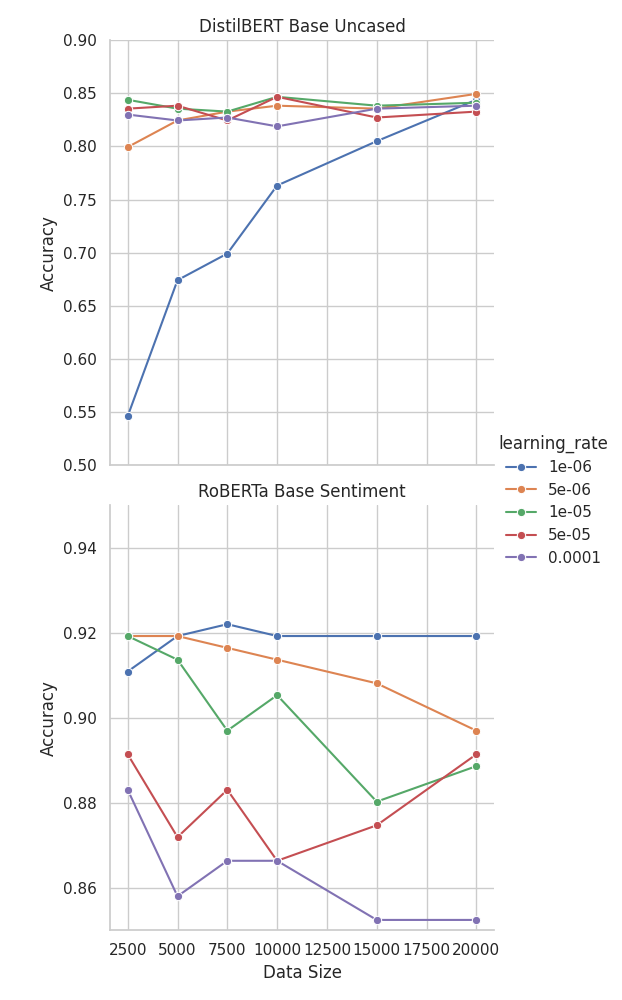
\includegraphics[height=0.7\textheight, keepaspectratio]{fine_tuning_results_bert_based.png}

  \vspace{0.3cm}
  \small
  Die Grafik zeigt die Genauigkeit von \textbf{DistilBERT Base Uncased} und \textbf{RoBERTa Base Sentiment}
  in Abhängigkeit der Datenmenge und Lernrate.
\end{frame}

\begin{frame}{Ergebnisse}
  \centering
  \small

  \vspace{0.3cm}
  \renewcommand{\arraystretch}{1.1}
  \setlength{\tabcolsep}{4pt}

  \resizebox{\textwidth}{!}{
      \begin{tabular}{p{3.8cm}|p{2.4cm}|p{2.4cm}|p{2.4cm}|p{2.4cm}}
          \hline
          \multicolumn{5}{c}{\textbf{DeepSeek-Modell:}} \\
          \hline
          \textbf{Modell} & \textbf{Daten-Größe} & \textbf{Lernrate} & \textbf{Genauigkeit} & \textbf{F1-Score} \\
          \hline
          DeepSeek-R1-Qwen & 10000  & 1e-5  & 0.866  & 0.866 \\
          DeepSeek-R1-Qwen & 7500   & 1e-5  & 0.855  & 0.855 \\
          DeepSeek-R1-Qwen & 5000   & 1e-5  & 0.855  & 0.855 \\
          DeepSeek-R1-Qwen & 20000  & 5e-6  & 0.852  & 0.852 \\
          DeepSeek-R1-Qwen & 15000  & 1e-5  & 0.852  & 0.852 \\
          DeepSeek-R1-Qwen & 10000  & 5e-6  & 0.850  & 0.850 \\
          DeepSeek-R1-Qwen & 7500   & 5e-6  & 0.849  & 0.849 \\
          DeepSeek-R1-Qwen & 5000   & 5e-6  & 0.847  & 0.847 \\
          DeepSeek-R1-Qwen & 20000  & 1e-6  & 0.846  & 0.846 \\
          DeepSeek-R1-Qwen & 15000  & 5e-6  & 0.845  & 0.845 \\
          \hline
      \end{tabular}
  }

  \vspace{0.3cm}
  \tiny
  Die Tabelle zeigt die besten durchläufe des DeepSeek-R1-Qwen-Modells nach Genauigkeit und F1-Score.

\end{frame}

\begin{frame}{Ergebnisse}
  \centering
  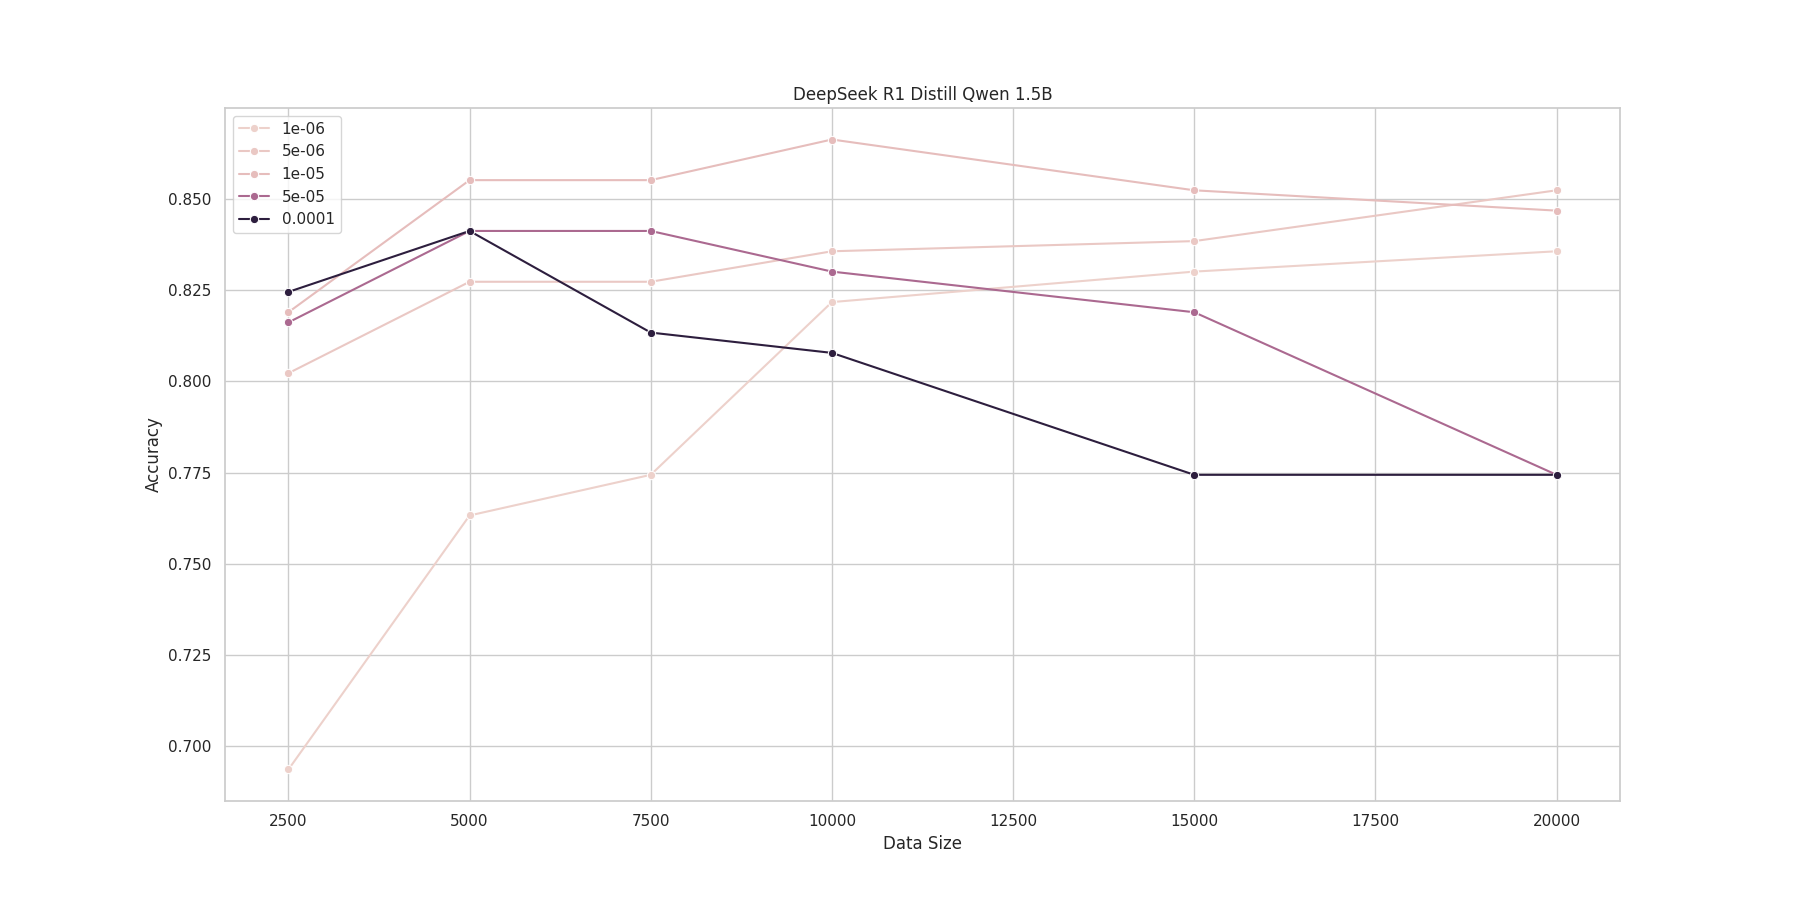
\includegraphics[width=0.85\textwidth, keepaspectratio]{fine_tuning_results_deepseek.png}

  \vspace{0.3cm}
  \small
  Die Grafik zeigt die Genauigkeit von \textbf{DeepSeek-R1-Distill-Qwen}
  in Abhängigkeit der Datenmenge und Lernrate.
\end{frame}

\begin{frame}{Ergebnisse}
  \Large
  \textbf{Einschränkungen beim Fine-Tuning großer DeepSeek-Modelle:}

  \vspace{0.5cm}

  \begin{itemize}
      \item Fine-Tuning größerer \textbf{DeepSeek-Modelle} war aufgrund hoher Hardware-Anforderungen nicht möglich.
      \item Speicher- und Rechenkapazitäten reichten für diese Modelle nicht aus.
      \item Daher wurde für große DeepSeek-Modelle ein \textbf{Zero-Shot-Ansatz} gewählt.
      \item Modelle wurden ohne Training direkt auf Testdaten evaluiert.
      \item So konnte ihre Leistungsfähigkeit trotzdem verglichen werden.
  \end{itemize}

\end{frame}

\begin{frame}{Ergebnisse}
  \Large
  \textbf{DeepSeek-R1-1.5B:}

  \vspace{0.5cm}
  \begin{itemize}
      \item \textbf{Genauigkeit:} 88,3 \% (mit Query), 82,4 \% (ohne Query)
      \item \textbf{F1-Score:} Negative: 0.885, Positive: 0.881
      \item Bessere Ergebnisse bei Einbeziehung des Suchbegriffs.
      \item Problematische Fälle: Tweets mit gemischten Emotionen oder Ironie.
  \end{itemize}
\end{frame}

\begin{frame}{Ergebnisse}
  \Large
  \textbf{DeepSeek-R1-8B:}

  \vspace{0.5cm}
  \begin{itemize}
      \item \textbf{Genauigkeit:} 95,5 \% (mit Query), 91,6 \% (ohne Query)
      \item \textbf{F1-Score:} Negative: 0.955, Positive: 0.956
      \item Deutlich bessere Erkennung von negativen und positiven Sentiments.
      \item Falsche Klassifikationen oft bei Mehrdeutigkeiten („beste Athlet“ vs. „beste aller Zeiten“).
  \end{itemize}
\end{frame}

\begin{frame}{Ergebnisse}
  \Large
  \textbf{DeepSeek-R1-32B:}

  \vspace{0.5cm}
  \begin{itemize}
      \item \textbf{Genauigkeit:} 96,7 \% (mit Query), 92,7 \% (ohne Query)
      \item \textbf{F1-Score:} Negative: 0.966, Positive: 0.967
      \item Fast fehlerfreie Erkennung bei Tweets mit klarem Sentiment.
      \item Schwächen bei Tweets mit Sarkasmus oder Wortspielen.
  \end{itemize}
\end{frame}

\begin{frame}{Ergebnisse}
  \Large
  \textbf{DeepSeek-R1-70B:}

  \vspace{0.5cm}
  \begin{itemize}
      \item \textbf{Genauigkeit:} 97,8 \% (mit Query), 93,0 \% (ohne Query)
      \item \textbf{F1-Score:} Negative: 0.977, Positive: 0.978
      \item Beste Performance unter den DeepSeek-Modellen.
      \item Bleibt bei Ironie, doppeldeutigen Tweets und Wortspielen fehleranfällig.
  \end{itemize}
\end{frame}








%=========================================================================================================================
\section{Zusammenfassung}

\begin{frame}{Zusammenfassung}
  \normalsize

  \begin{columns}[t]
    \column{0.47\textwidth}
      \textbf{Datenauswahl} \\[0.2cm]
      \begin{itemize}
          \item Sentiment140-Datensatz gewählt.
          \item Tweets bereinigt und Merkmale extrahiert.
      \end{itemize}

      \vspace{0.4cm}

      \textbf{Klassische Methoden} \\[0.2cm]
      \begin{itemize}
          \item Trainiert und evaluiert.
      \end{itemize}

      \vspace{0.4cm}

      \textbf{Deep Learning} \\[0.2cm]
      \begin{itemize}
          \item BERT- und DeepSeek-Modelle getestet.
          \item Größere Modelle liefern bessere Ergebnisse.
      \end{itemize}

    \column{0.47\textwidth}
      \textbf{Skalierbarkeit} \\[0.2cm]
      \begin{itemize}
          \item Fine-Tuning großer DeepSeek-Modelle nicht möglich.
          \item Zero-Shot-Ansatz genutzt.
      \end{itemize}

      \vspace{0.4cm}

      \textbf{Ausblick} \\[0.2cm]
      \begin{itemize}
          \item Fine-Tuning auf größeren Modellen prüfen.
          \item Optimierung bestehender Modelle.
      \end{itemize}

      \vspace{0.4cm}

      \pause

      {\large \textbf{Vielen Dank für Ihre Aufmerksamkeit!}} \\[0.1cm]
      \textit{Fragen?}

  \end{columns}

\end{frame}


\end{document}
